\documentclass[aspectratio=169]{beamer}              % only frames

% for themes, etc.
\mode<presentation>
\usetheme{Madrid} 
\usecolortheme{crane}

%\usepackage{times}  % fonts are up to you
% The usual suspects
\usepackage{multirow, booktabs, dcolumn, color, graphicx} % Tables\usepackage{graphicx}
\usepackage{amsmath,amssymb,amsthm}
% Strikethrough text
\usepackage{soul}
% Adjust box to fit tabulars
\usepackage{adjustbox}
% Embed video
\usepackage{media9}
% For notes
\usepackage{pgfpages}
%\setbeameroption{hide notes} % Only slides
%\setbeameroption{show only notes} % Only notes
\setbeameroption{hide notes} % Both
% Give a slight yellow tint to the notes page
%\setbeamertemplate{note page}{\pagecolor{yellow!5}\insertnote}\usepackage{palatino}
% Use colors by name
\usepackage{xcolor}
% EMBEDDING VIDEO IS POSSIBLE WITH PDFPC USE PDF PC to present
\usepackage{multimedia}



% The table highlighting for hypothesis discussion.
\usepackage[beamer,customcolors]{hf-tikz}
\usetikzlibrary{calc}

% To use background images
\newenvironment{colorframe}[2][]{%
\setbeamercolor{background canvas}{bg=#1}
\begin{frame}\color{white}}
{\end{frame}}


% To set the hypothesis highlighting boxes red.
\tikzset{hl/.style={
    set fill color=red!80!black!40,
    set border color=red!80!black,
  },
}

% Set Graphics folder
\graphicspath{{./figures/}}


% these will be used later in the title page
\title{Computer Networks}
\subtitle{Protocol Stack and Security}
\author{Irfan Kanat}
\institute[CBS]{{Department of Digitization}\\ Copenhagen Business School}
\date{\today}



\begin{document}

% this prints title, author etc. info from above
\begin{frame}

	\titlepage

\end{frame}

\note{In this video we will talk about how the protocol stack effects security.}


\begin{frame}
	\frametitle{Envelopes within envelopes...}

	\centering
    
  	\includegraphics<1>[width = \textwidth, height = .85\textheight, keepaspectratio]{figures/f1-4.png}

   	\includegraphics<2>[width = \textwidth, height = .85\textheight, keepaspectratio]{figures/envelopes.png}

\end{frame}

\note{
	We learned in the previous video that there was this protocol stack with different types of addressing in each layer. 

	This can be used both for attack and for defense.
}



\begin{frame}
	\frametitle{Networking and Security - Firewall}

	Least Functionality \vspace{1em}

	Allow traffic that fits function

\end{frame}

\note{
	Most attacks that come over the network work by exploiting an unpatched vulnerability in the server.

	One way to minimize this impact is to minimize the attack surface. Don't give access to services you don't absolutely need. This ties in with the ``Least functionality'' principle.

	Knowing the functionality of a computer, you can create rules for acceptable network traffic.
}


\begin{frame}
	\frametitle{Firewall}

	HTTP server: Allow TCP and UDP on Ports 80 and 443. \vspace{1em}

	SSH connection: Allow TCP port 22. \vspace{1em}

	The machine is a client? Do not allow incoming TCP SYN requests. \vspace{1em}

	The machine is a local server? Only allow traffic from local network. \vspace{1em}

	Connection is wired? Deny traffic on wlan interface \ldots

\end{frame}


{
\usebackgroundtemplate{
\includegraphics[width=\paperwidth,height=\paperheight]{demoland.png}}%
	\begin{frame}
	\frametitle{UFW Firewall}



	\end{frame}
}

\note{
	I set up an AWS instance for this demo. Look up its IP address before you begin.

	1 - Show which ports are open on a computer with nmap

	2 - Try to feed ip into a browser and get no result

	3 - Log into the server.

	4 - Change firewall settings to allow HTTP traffic

		sudo ufw status

		sudo ufw enable 80

	5 - Get back to your own machine and do another port scan show 80 now open for business

	6 - Show in browser the hello friend page.

	Other rules for purposes.

	Deny certain networks

		sudo ufw deny from 15.15.15.0/24

	Allow SSH?

		sudo ufw allow ssh

	A series of rules carried out in order

		sudo ufw status numbered

	Show which ports are open with nmap

}



\begin{frame}
	\frametitle{Spoofing}
    
	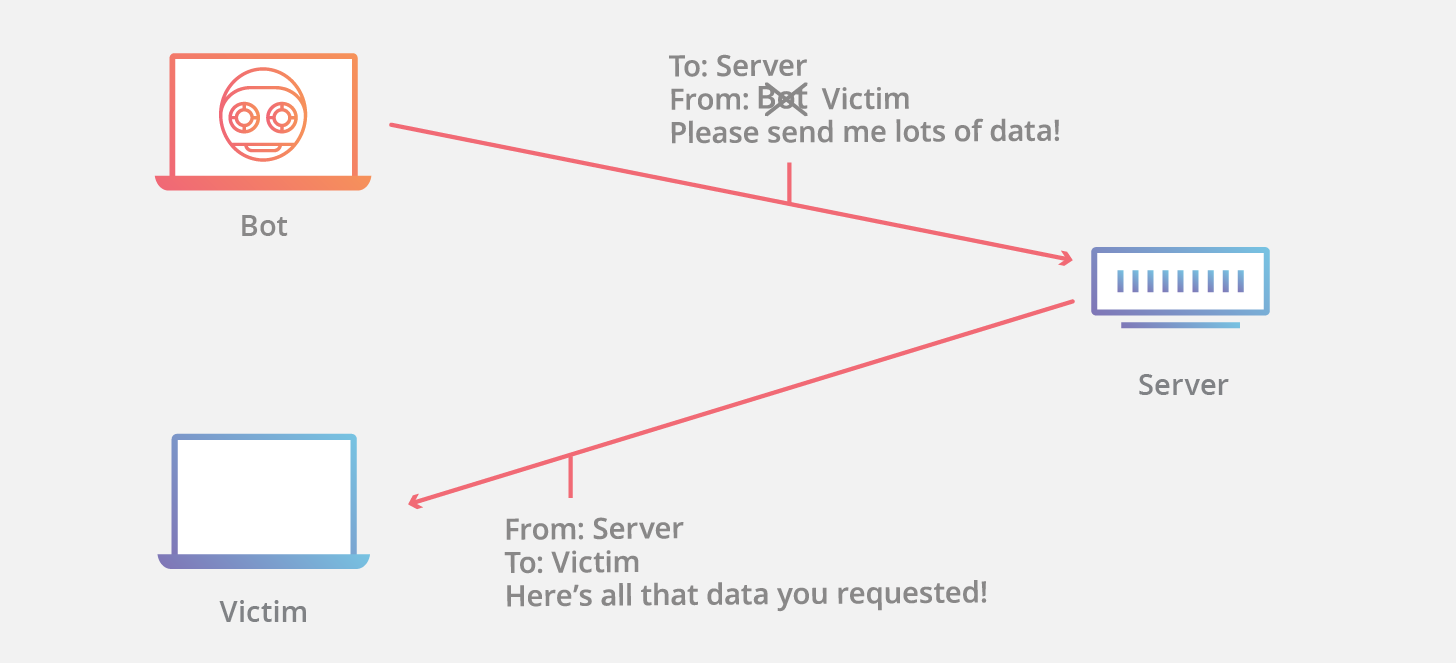
\includegraphics[width = \textwidth, height = .85\textheight, keepaspectratio]{figures/0.0.png}

\end{frame}

\note{
	Many different kinds of spoofing exist.

	Mail spoofing, MAC address spoofing, IP spoofing.

	It essentially means pretending to be someone you are not.

	In case of IP spoofing, it is very useful in multiplying your DDoS capability.

	Make a small request to a server with a large return package. Plug victim IP as source IP. Now for every small package you sent, victim will receive a large package. Used in DNS amplification attacks.
}





\end{document}
